\documentclass[a4paper]{article}

\usepackage[T1]{fontenc}                % För svenska bokstäver
\usepackage[swedish]{babel} 
\usepackage{graphicx}            % För svensk avstavning och svenska
                                        % rubriker (t ex "innehållsförteckning)


\def\code#1{\texttt{#1}}

\title{News System \\
 EDA031 Project }
\author{Erik Stenlund, Alexander Karlsson, Kit Gustavsson, Erik Nimmermark}


\begin{document}

\maketitle                      % Titel hamnar på en egen sida. Detta
                                % kan man även få med klassen article
                                % om man anger optionen "titlepage":
                                % \documentclass[titlepage,a4paper]{article}

% Den stora skillnaden mellan artikel och rapport är att den senare
% har en ytterligare rubriknivå, nämligen "chapter".
%
% Varje kapitel börjar på en ny sida. Cirka en tredjedel ner på sidan
% står det följande text i stora bokstäver:
%
%      Kapitel 1.
%      Sammanfattning
%
% Om man använder report men glömmer att det finns en rubriknivå som
% heter \chapter och bara använder \section kommer det första stycket
% att heta 0.1
%
% Denna dokumentklass lämpar sig därförr bäst för mycket stora
% dokument. För det mesta duger article bra.

     % Kapitel 1
                                % Sammanfattning
\newpage
\section{System Design}
\subsection{Description and responsibilities of classes}             % 1.1 inledning
\subsubsection{Classes used by server}
\code{BestServer}\newline
This program has the main method for the primary memory server and  is the server that use primary memory to store the newsgroups and articles. It uses a \code{Server} object to start the server and communicate with connected clients using a \code{MessageHandler}. The server reads the messages that follows the given protocol and handles the commands, given by \code{Protocol} that is received from the client. For storing of the data the \code{BestServer} contains an object of the class \code{MemoryDatabase}.
\newline \newline
\code{DiscServer}\newline
This program has the main method for the hard drive server and is a server that stores newsgroups and articles on the hard drive. It uses a \code{Server} object to start the server and then handles the communication with the connected clients using a \code{MessageHandler}. It works the same way as the \code{BestServer} but uses a \code{DiscDatabase} instead of the \code{MemoryDatabase} for storage of the data. 
\newline \newline
\code{Database}\newline
This is the superclass of the \code{DiscDatabase} and the \code{MemoryDatabase} and it contains virtual members that handle adding, removing and accessing newsgroups and articles. It also contains a private attribute that decides which the next newsgroup ID to be used is. The header file also contains structs that represents both the articles and the newsgroups that are used throughout the server programs. The newsgroup struct contains a map which contains all the articles in that specific newsgroup, the map uses the article id as key.
\newline \newline
\code{DiscDatabase}\newline
The \code{DiscDatabase} class extends the \code{Database} class and uses the hard drive for storing the newsgroups. At start-up it check if the folder named root exists in the directory of the program. If not it creates it, the root folder is used to store the database on the hard drive. If the root folder exists the program creates newsgroup structs for each sub-folder in root and article structs for all files in the sub-folders. To decide which id a new newsgroup or article should have each folder contains a file called nextID which contains the next id for the article if it is in a sub-folder or the next id for the newsgroup if it is in the root folder. The class also has member functions for adding, removing and accessing articles or newsgroups from the database.
\newline \newline
\code{MemoryDatabase}\newline
This class also extends the \code{Database} class and uses the memory for storing the newsgroups and articles which means that they won't be saved when closing the server. The class uses a map for storing the newsgroups structs using the id as key. It has members for accessing, inserting and removing newsgroups from the list and for accessing, inserting and removing articles from a newsgroup.
\subsubsection{Classes used by client}

\code{Client}\newline
This is the class with the main method on the client side. The main sets up the connection and listens to user input. Depending on what command, from \code{Protocol}, the user typed it send the correct command (according to the protocol) to carry out what the user intended to do or prints an error message if it cannot be done for some reason.
All the communication between the client and the server is sent using the \code{MessageHandler} class.
 
\subsubsection{Classes used by both server and client}
\code{Protocol}\newline
Class with all the enums for the different flags a message can contain. This is used to get rid of magic numbers in the code and make it easier to understand.
\newline \newline
\code{Messagehandler}\newline
The class that is responsible for sending the data between the server and the client. The methods contains the logic for receiving and sending bytes in different ways depending on that kind of message that is to be sent/received. It uses the \code{Connection} class to actually send and receive bytes of data.
\newline \newline
\code{Connection}\newline
The class that represents the connection with socket and address. This is that class that writes and reads data. The methods for sending and receiving data is used by the \code{MessageHandler} class to actually send and receive data between the client and server.
\section{Conclusion}            % Kapitel 2
Our programs do fulfil all the given requirements from the specification. The client both reads and present input and server replies to and from the terminal. The client program command help gives all information about how to use the program and all errors are handled and prints an error message to the clients terminal window.\newline \newline We have got two different server version, one using the primary memory and one using the hard drive. Both our Databases guarantee that each newsgroup has an unique id number and that the article id are unique for each newsgroup, this is done using files containing the next id described earlier. The newsgroups and articles are ordered using the id number which is incremented for each new newsgroup and article. This makes the articles and newsgroups listed in chronological order. The servers also handles as many (as long as there is memory) newsgroups and articles as possible with as long titles as possible. 
\newline \newline
One problem with our DiscDatabase is that it reads all information in the database on the hard drive once each start-up. That means that removing needed files on the hard drive during execution of the server would not be seen by clients connected to the server. We see this actions as incorrect use of the server and the one editing the database files should be held responsible in that case.

\newpage
\section{UML and Sequence diagrams}
\begin{figure}[h]
    \centering
    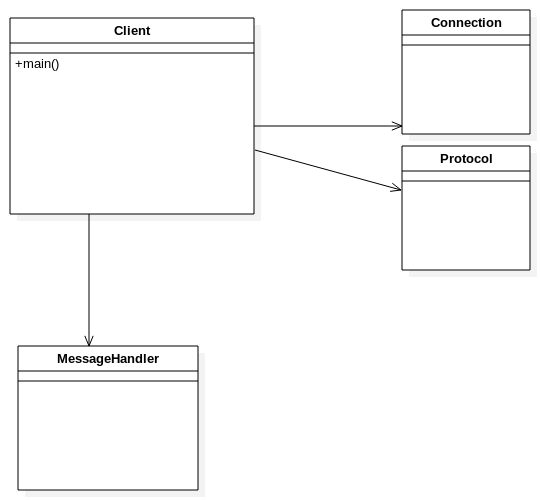
\includegraphics[width=\textwidth]{clientUML.png}
    \caption{UML for Client program}
    \label{fig:awesome_image}
\end{figure}


\begin{figure}[h]
    \centering
    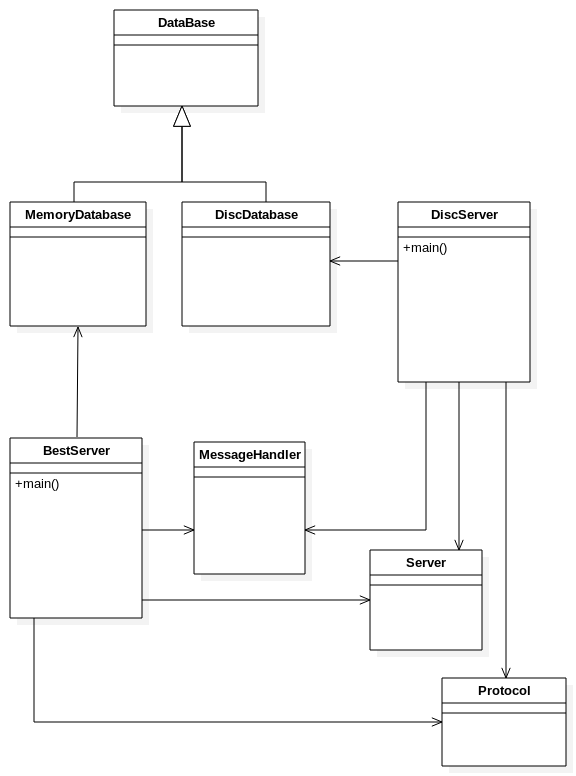
\includegraphics[width=\textwidth]{serverUML.png}
    \caption{UML for Server programs}
    \label{fig:awesome_image}
\end{figure}
\newpage
%\section{Server dynamics}
%\subsection{Sequence diagram}

\begin{figure}[h]
    \centering
    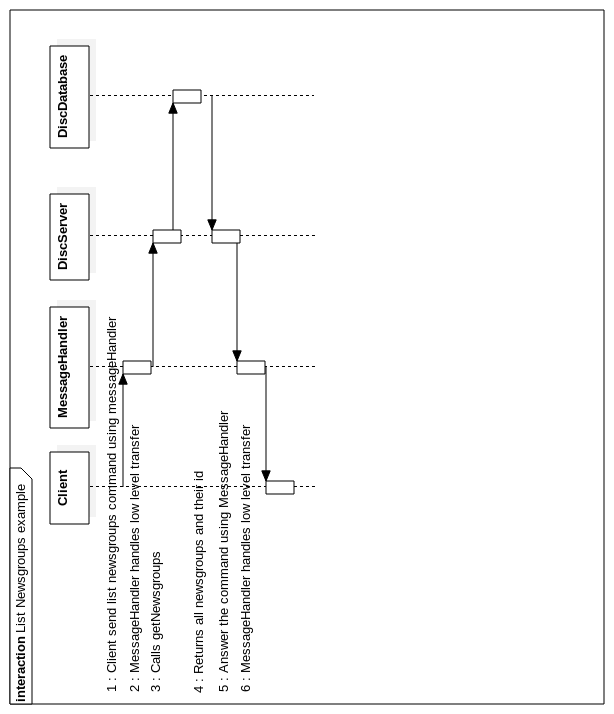
\includegraphics[width=\textwidth]{listnewsgroups90.png}
    \caption{Sequence diagram for List Newsgroups command}
    \label{fig:awesome_image}
\end{figure}
\newpage

\end{document}
